\documentclass[8pt, letterpaper]{article}
\usepackage{graphicx}
\usepackage[utf8]{inputenc}
\usepackage{gensymb}
\usepackage{pgfplots}
\usepackage{tikz}

\graphicspath{{images/}}
\pgfplotsset{compat = newest}

\setlength{\parindent}{0cm}

\title{Auswirkung der Auslenkung auf die Schwingdauer eines Fadenpendels}
\author{
	Jakob Kirsch \and
	Felix Warschburger \and
	Manjaap Singh \and
	Luca Clemens \and
	Rogier Van de Veen
}

\begin{document}
\maketitle

\section{Fragestellung (Felix)}
Besteht eine Korrelation zwischen der Auslenkung und der Schwingdauer eines Fadenpendels?

\section{Versuchsbeschreibung (Manjaap)}
Wir haben uns zu fünft verschiedene Aufgaben gegeben:
\begin{itemize}
  \item Eine Person zählt die Schwingungen und misst die Größe, als das Fadenpendel losgelassen wurde, um dessen Auslenkungswinkel zu bestimmen
  \item Drei Personen messen jeweils die Dauer der Schwingung
  \item Eine Person notiert die Zeiten, die von den anderen 3 gemessen wurden
\end{itemize}

\section{Aufbau (Luca)}
\begin{center}
  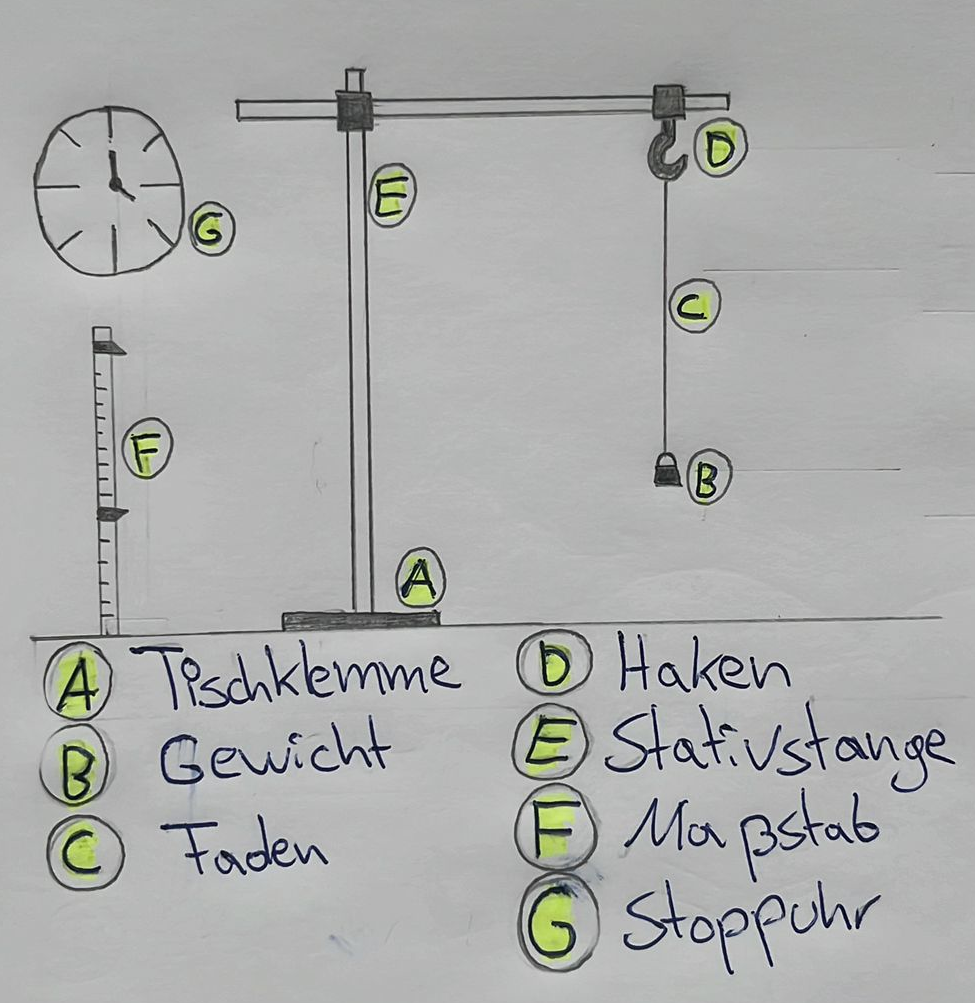
\includegraphics[width=8cm]{image1}
\end{center}

\section{Durchführung (Rogier)}
Um die Winkel deterministisch zu halten, wird das Pendel innerhalb eines Versuches immer von der selben Höhe losgelassen.
Die Winkel lassen sich mit $arccos(\frac{h_a - h_p}{l})$ errechnen, wobei $h_a$ die Höhe des Pendels, also vom Boden bis zur Befestigung, $h_p$ die Höhe, von der das Fadenpendel losgelassen wurde, und $l$ die Länge des Fadenpendels darstellt.

Es werden 4 Messdurchgänge durchgeführt, wodurch 12 Messwerte pro Versuch entstehen.
Jeder Messwert entspricht 10 Schwingungen, um eventuelle Ungenauigkeiten zu minimieren.

\section{Messergebnisse (Felix)}
\begin{center}
  \begin{tabular} { c|c|c|c }
    Wert & Versuch 1 & Versuch 2 & Versuch 3 \\
    \hline
    01 & 25.74 & 24.80 & 24.18 \\
    02 & 25.53 & 24.66 & 24.38 \\
    03 & 25.65 & 24.94 & 24.61 \\
    04 & 25.44 & 24.84 & 24.19 \\
    05 & 25.51 & 24.84 & 24.35 \\
    06 & 25.61 & 24.82 & 24.25 \\
    07 & 25.41 & 24.74 & 24.39 \\
    08 & 25.45 & 24.84 & 24.38 \\
    09 & 25.43 & 24.93 & 24.35 \\
    10 & 25.36 & 24.90 & 24.49 \\
    11 & 25.45 & 24.80 & 24.49 \\
    12 & 25.59 & 24.98 & 24.06
  \end{tabular}
\end{center}

Die Winkel der Auslenkung für die Versuche sind 60.45\degree, 45.9\degree und 25.01\degree
Aufgrund von einer Änderung der Vorgehensweise der Zeitmessung bei Versuch 2 und 3 im Vergleich zu Versuch 1 sind die Werte skeptisch zu betrachten.

\section{Auswertung (Jakob)}
Aus der Tabelle ergeben sich folgende Werte:
\begin{center}
  \begin{tabular} { c|c|c|c }
    Veruch & 1 & 2 & 3 \\
    Durchschnitt & 25.51 & 24.84 & 24.34 \\
    Median & 25.48 & 24.84 & 24.365 \\
    Mittlere Abweichung $\sigma$ & 0.108 & 0.085 & 0.148 \\
    Min & 25.36 & 24.66 & 24.06 \\
    Max & 25.74 & 24.98 & 24.61
  \end{tabular}
\end{center}

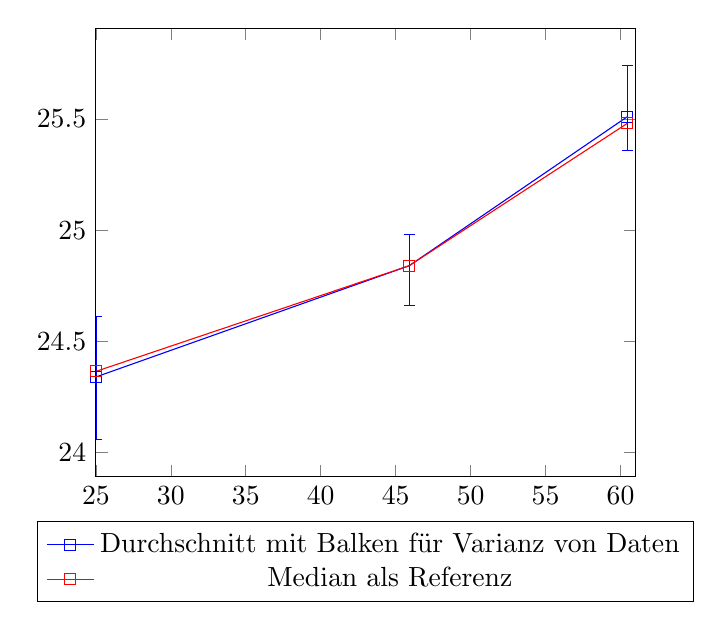
\begin{tikzpicture}
  \begin{axis}[xmin = 25, xmax = 61, legend style={at={(0.5,-0.1)},anchor=north}]
    \addplot[
      color=blue,
      mark=square,
      error bars/.cd,
        y fixed,
        y dir=both,
        y explicit
    ] table[x=x, y=y, y error plus=y-max, y error minus=y-min, col sep=comma] {
      x, y, y-max, y-min
      60.45, 25.51, 0.23, 0.15
      45.9, 24.84, 0.14, 0.18
      25.01, 24.34, 0.27, 0.28
    };

    \addplot[
      color=red,
      mark=square
    ] coordinates { (60.45,25.48)(45.9,24.84)(25.01,24.365) };

    \addlegendentry{ Durchschnitt mit Balken für Varianz von Daten }
    \addlegendentry{ Median als Referenz }
  \end{axis}
\end{tikzpicture}

\section{Interpretation (Jakob)}

\subsection{Ansatz 1}
Anhand des Verlaufes der Dauer einer Schwingung in Relation zur Auslenkung ist darauf zu schließen, dass die Auslenkung einen Einfluss auf die Dauer einer Schwingung eines Fadenpendels hat.
Aufgrund des Mangels an verschiedenen Messungen ist es leider nicht möglich, den Typ der Korrelation zu bestimmen. Hier ein paar Beispiele:

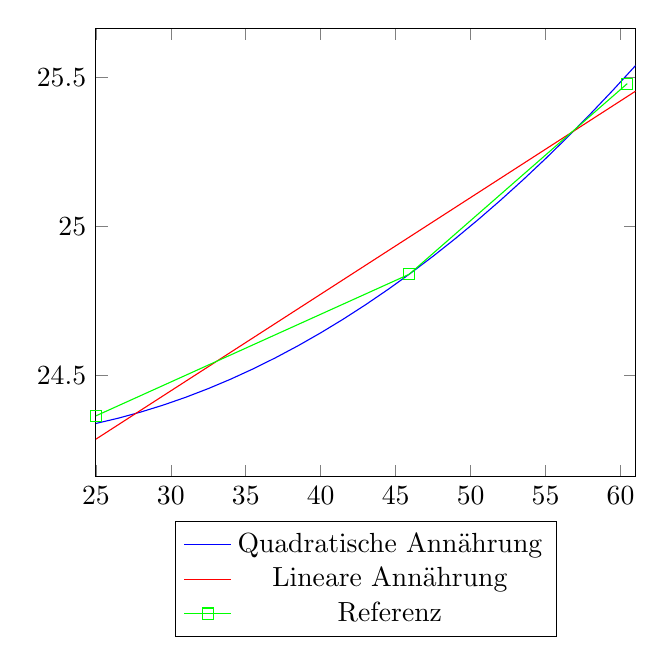
\begin{tikzpicture}
  \begin{axis}[xmin = 25, xmax = 61, legend style={at={(0.5,-0.1)},anchor=north}]
    \addplot[
      color=blue,
      domain=25:61
    ] { 0.000623071 * x * x - 0.0202155 * x + 24.4552 };

    \addplot[
      color=red,
      domain=25:61
    ] { 0.0324445 * x + 23.4754 };

    \addplot[
      color=green,
      mark=square
    ] coordinates { (60.45,25.48)(45.9,24.84)(25.01,24.365) };

    \addlegendentry{ Quadratische Annährung }
    \addlegendentry{ Lineare Annährung }
    \addlegendentry{ Referenz }
  \end{axis}
\end{tikzpicture}

\subsection{Ansatz 2: Bedenken an Wertgenauigkeit}
Da das Verhältniss der Auslenkung zwischen Versuch 1 und Versuch 3 bei 0.43, das Vehältniss der Werte aber bei 1.05 liegt, kann man davon ausgehen, dass durch den menschlichen Faktor sich auch Ungenauigkeiten eingeschlichen haben, welche auf eine falsche Korrelation hindeuten würden.
Es besteht der Bedarf nach genaueren Messungen mit mehr Auslenkungen und genaueren (Computer gestützten) Messgeräten.

\subsection{Vermutung}
Man könnte vermuten, dass die Energiedifferenz eines Punktes von vor und nach einer Schwingung unter Vernachlässigung des Luftwiderstandes, der Reibung und jeglicher anderen externen Einflüssen 0 beträgt, da die aufzubringende Energie die freigewordene Energie ausgleicht, da die potentielle Energie eines Punktes immer gleich ist. Da ein Objekt zwar bei längerem Fall mehr Geschwindigkeit aufbaut, aber auch weiter auf der anderen Seite schwingen muss, neutralisiert sich die Diskrepanz der Zeit wahrscheinlich. Es besteht wie gesagt Bedarf nach weiteren Versuchen.

\end{document}
